%%%%%%%%%%%%%%%%%%%%%%%%%%%%%%%%%%%%%%%%%%%%%%%%%%%%
%%%% En-tête leçon
\begin{headerBlock}
  \chapter{Traitement d'un signal. Etude spectrale.}
    \label{LP_TraitementSignal}
\end{headerBlock}

%%%%%%%%%%%%%%%%%%%%%%%%%%%%%%%%%%%%%%%%%%%%%%%%%%%%
%%%% Références
\begin{center}
\begin{tabularx}{\textwidth}{| X | X | c | c |}
  \hline
  \rowcolor{gray!20}\multicolumn{4}{c}{Bibliographie de la leçon : } \\
  \hline 
  Titre & Auteurs & Editeur (année) & ISBN \\
  \hline
  Electronique & Pérez & Dunod &   \\
  \hline 
  Traitement des signaux et acquisition de données & Francis Cottet & Dunod & 2-10-006312-X \\
  \hline 
  Tout-en-un PSI &  & Tec\&Doc & \\
  \hline
  Dictionnaire de physique & R. Taillet, L. Villain, P. Febvre & de Boeck & \\
  \hline
  Cours Jérémy Neveu & J. Neveu & & \\
  \hline
\end{tabularx}
\end{center}

%%%%%%%%%%%%%%%%%%%%%%%%%%%%%%%%%%%%%%%%%%%%%%%%%%%%
\begin{reportBlock}{Plan détaillé}
  \textbf{Niveau choisi pour la leçon :} 
  \newline
  \textbf{Prérequis : }
  \newline

\section*{Introduction}
\textcolor{red}{Accroche : (cf cours Jérémy Neveu) }L'enjeu des communications est de pouvoir envoyer un signal (\textit{i.e.} une information) depuis un émetteur jusqu'à un récepteur afin que celui-ci puisse être d'une part reçu et d'autre part compris.
\begin{center}
    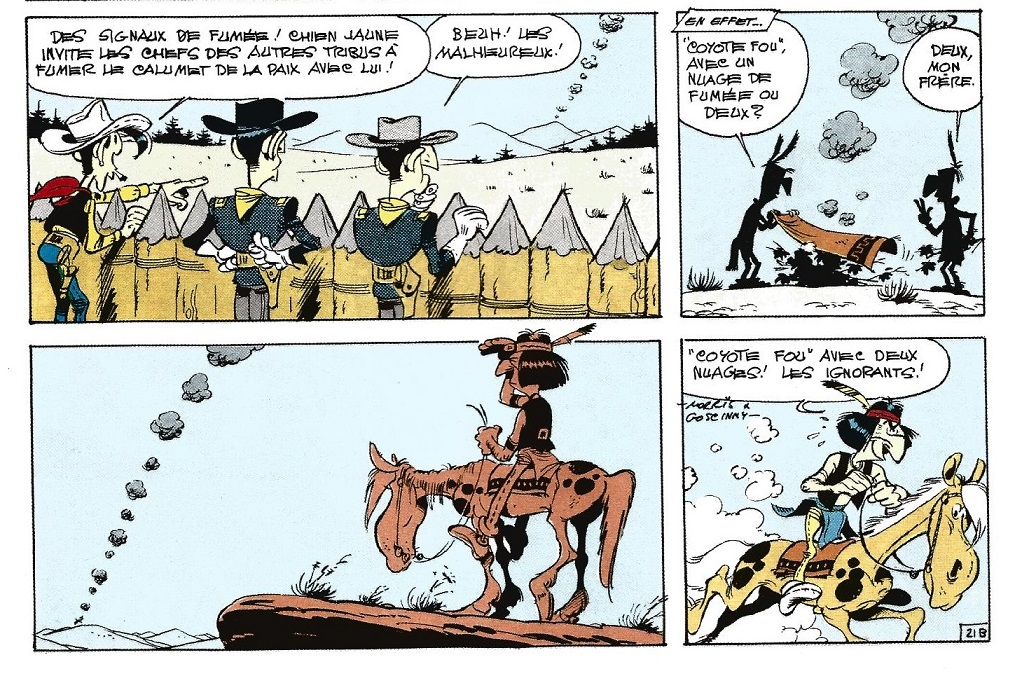
\includegraphics[scale=0.8]{LP_TraitementSignal/Codage_LuckyLuke.jpg}
\end{center}
\textcolor{green}{signal :} (ref Taillet p674) Variation temporelle ou spatiale d'une quantité physique mesurable (tension, force, lumière, ...) portant une information.\\
\textcolor{green}{Traitement du signal :} Transformation d'un signal reçu par un récepteur pour en retirer l'information transmise initialement par un émetteur. Ex : si un observateur cherche à analyser la lumière émise par une étoile (\textcolor{green}{signal}) à travers l'atmosphère, il doit se séparer de celle émise par l'atmosphère (\textcolor{green}{bruit}) par différents moyen (filtrage par exemple).

\section{Spectre et filtrage d'un signal}

\subsection{Décomposition Fourier}
Tout signal peut se décomposer comme une série de signaux sinusoïdaux.\\

Spectre d'énergie d'un signal cf Cottet : composante continue, fondamental, harmoniques.\\

Propriétés TF (?) et principe de la FFT sur un oscillo (pour préparer les mesures de la deuxième partie)

\subsection{Types de signaux}
Signaux analogiques vs numériques. On va se concentrer sur les signaux analogiques.


\subsection{Réponse d'un filtre RC à une excitation périodique}
Prendre l'exemple d'un circuit RC passe-bas (mesure sur la capa), tracer le diagramme de Bode et déterminer la fréquence de coupure $f_c = \frac{1}{RC}$. Mettre en évidence le $-20\log(\omega)$.

\subsection{Autres types de filtre}
\textbf{Transition :} Maintenant qu'on a décrit un signal et qu'on s'est en retirer des informations, on va voir comment en envoyer un et comment le réceptionner.

\section{Modulation et démodulation en amplitude}
Fil conducteur : radio analogique. Cf cours de Jérémy.
Deux problèmes : 
\begin{itemize}
    \item \textcolor{green}{l'encombrement :} deux personnes qui parlent en même temps,
    \item dimension des antennes : longueur de l'antenne doit être de l'ordre de la longeur d'onde soit 1500km pour $f=20Hz$ et 1.5km pour $f=20000Hz$ ...
\end{itemize}

\subsection{Principe de la modulation en amplitude}
On souhaite passer à des tailles d'antennes raisonnable de l'ordre du mètre : soit $f=\frac{c}{\lambda}=30$MHz : c'est le principe de la modulation.

\textcolor{green}{Modulation :} Accrocher un signal à transmettre à une porteuse : modulation de la porteuse. Ex : pigeon voyageur (porteuse) pour faire passer une lettre (signal modulant) d'un point A à un point B\\

Pour un signal EM : 
\begin{itemize}
    \item $V_m(t)=A+B\cos(\omega_mt)$ pour la modulation
    \item $V_p(t) = V_0\cos(\omega_pt)$
\end{itemize}

Introduction signal modulant ou à transmettre (GBF Agilent 500Hz : le message à faire passer) porteuse (BGX Métrix à 50kHz : le pigeon voyageur)\\

Qualité de la transmission : spectre, bruit, rapport signal à bruit

\subsection{Démodulation par détection synchrone}
\textcolor{red}{Attention :} pour que ça puisse fonctionner, il faut que la porteuse puisse être regénéré (on peut le faire avec une boucle à vérouillage de phase, le mentionner peut-être en conclusion de la partie).\\

\textcolor{blue}{Manip : démodulation par détection synchrone}. Le TP est bien fait, montrer le signal qu'on module, le signal après multiplication par la porteuse et le signal après le filtre passe-bas.



\end{reportBlock}